\section{Overview}

This chapter will explain the general concept and architecture of the traffic light control system developed with this thesis. The traffic light control system will be built upon an existing traffic simulation, because the thesis is not about the simulation, but the optimization of the traffic light control. Which simulation is chosen will be discussed in a later section of the thesis and is not really relevant here, but this architecture will influence which traffic simulation will be chosen. The requirements for the traffic simulation will be derived from this concept.

\begin{figure}[ht]
  \centering
  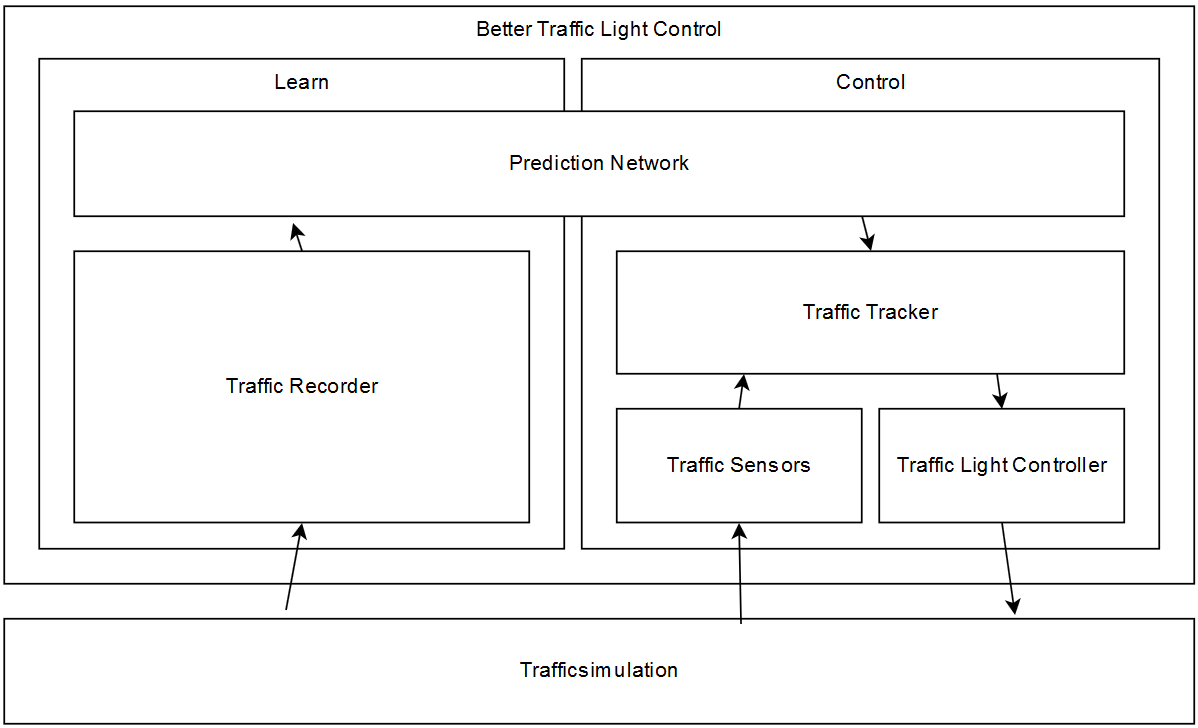
\includegraphics[width=16cm]{figures/architecture}
  \caption[Architecture of the Traffic Light Control System]{Architecture of the Traffic Light Control System \protect\footnotemark}
  \label{architecture}
\end{figure}

\footnotetext{own illustration}

The traffic light control system is separated into general areas, the learning part of the system and the controlling part. Either the system just observes a running traffic simulation and learns the patterns of the traffic or it observes the simulation through traffic sensors and controls the traffic lights according to the predictions combined with the data from the traffic sensors. It is imaginable to let the system learn from a simulation and control it at the same time, but this is outside of the scope of this thesis. But it could possibly improve the results and make it more practicable for a real world deployment.

The control part of the system is the more important. The learning is relatively simple and will be easily interchangeable. This is also the reason why the architecture was split into two parts. With the simulation the data to learn from will be recorded from the simulation itself, but in a real world scenario data could also be fed from other sources, thus the data collection in the learning part is not a main feature of the traffic light control system and was split from the core control part.

Spanning both the learning and the control part of the system is the prediction network. It is responsible for actually learning the traffic behavior and feeding predictions of the learned behavior back into a real simulation. For this task the prediction network will include an artificial neural network or multiple of them in some form, which is detailed in section \ref{predictionNetwork}. The prediction network will use unsupervised learning to learn the traffic patterns, meaning that there will not be labeled data sets collected beforehand or a continuous interaction with the simulation, but the data sets will be collected from a running traffic simulation.

The traffic recorder will collect such data sets and feed them into the prediction network. Depicted in figure \ref{architecture} is only the default implementation of the traffic recorder which collects the data sets directly from the traffic simulation. The design goal of this component is to split the learning set creation and handling from the prediction network to be flexible and extensible in how data is fed to the prediction network. The default implementation will observe the state of the traffic network and record the data that is compliant to the prediction networks input and output formats. With the component split from the prediction network the creation of data sets is clearly separated from the prediction network. Thus it is, as said earlier, possible to change the way data is fed to the prediction network easily. In a real world scenario it probably would be nearly impossible to automatically record the data sets and it would be a huge benefit to easily swap out the learning input to some other method, which is totally possible with this architecture.

In the control part of the system the interaction with the traffic simulation occurs over traffic sensors that collect data and the traffic light controller that switches the states of the traffic lights. The different traffic sensors that are commonly used already are detailed in section \ref{trafficSensors}. Depending on the traffic simulation software chosen later, they are already part of the simulation or have to be simulated by observing the state of the simulation an extracting the relevant information. The data they need from the simulation and the data they pass on to the next component depends on the type of sensor used. An induction loop may only report if a vehicle currently is on top of it or not, but a camera attached to the traffic light might even count the amount of vehicles waiting for the light to turn green. The traffic light controller has to switch the traffic lights depending on the input he gets from the traffic tracker and is further described in section \ref{trafficLightController}. Like the traffic recorder the goal here was to be able to swap out the layer communicating information to the main components of the traffic light control system. An additional goal for the traffic light controller was to be able to swap out the strategy that it uses to control the traffic lights, but this is discussed in more detail in section \ref{trafficLightController}.

The final component of the architecture is the traffic tracker that keeps all other components together. Its task is to use the prediction network and the traffic sensors to create a picture of reality that has to closely match what is really happening. The traffic tracker can then make a statement about where cars should be in the system an the traffic light controller can then, based upon the traffic trackers data, make decisions how the traffic lights have to be optimally switched. The difficulties arising in this component are various. For example, a traffic sensor could discover that a  prediction made by the prediction network is wrong. This has to be corrected somehow, but with a complex street network it may not be easy to detect where the failure came from. This problem is from now on called the error correction problem. Furthermore traffic sensors may give very vague or heterogeneous data, making it hard to incorporate the data into the picture of reality.

\begin{figure}[ht]
  \centering
  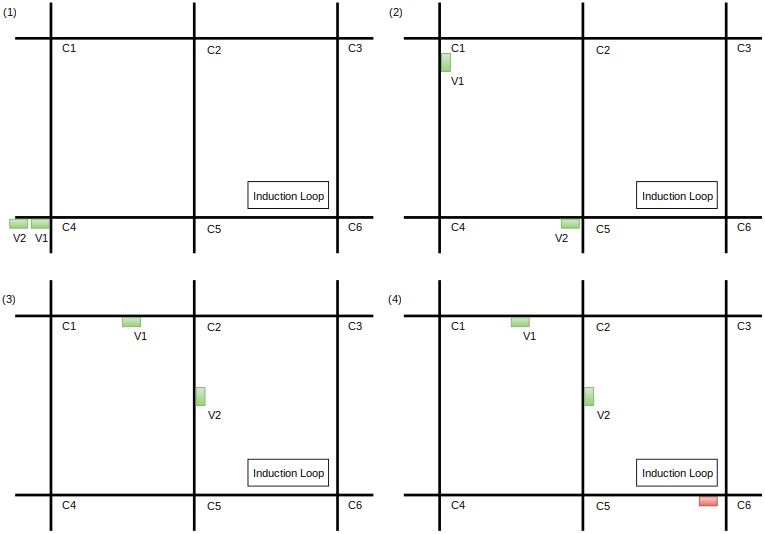
\includegraphics[width=16cm]{figures/errorCorrectionProblem}
  \caption[Error Correction Problem]{Error Correction Problem \protect\footnotemark}
  \label{errorCorrectionProblem}
\end{figure}

\footnotetext{own illustration}

Figure \ref{errorCorrectionProblem} shows an example for the error correction problem. In this example two vehicles V1 and V2 depicted in green entered at the road crossing C4. (1) Here the first prediction was that one car drives to C1 and the other one drives to C5. (2) This prediction is only based on the learned traffic patterns and could be completely wrong, but should in the most cases be right.

When V1 enters crossing C1 the prediction is that it drives to C2. The prediction for V2 is that it continues from C5 to C2. (3) In the example, crossing C6 is equipped with induction loops and detects when a vehicle enters the crossing.

Finally a vehicle is detected at C6, but in the traffic tracker all vehicles in the network are at other positions and no vehicle was predicted to drive there. This is not trivial to solve and could be solved in many different ways. Either V1 or V2 could be predicted wrong. The correction, if V2 would be wrong, is straight forward. V2 is just moved to the crossing, but if V1 is chosen to be moved there, it could have had implications on the prediction at crossing C5, where the prediction was made with one vehicle, but should then have been made with two. This could then spawn new errors in the network that would have to be resolved.

With this really simple example alone one can see how it is difficult to resolve errors in a complex network that are detected by traffic sensors. With more vehicles and more crossings the problem gets even bigger. A solution algorithm for these problems will be implemented by the traffic tracker which is discussed in more detail in section \ref{trafficTracker}.

With this architecture it should be possible to experiment with different traffic sensors and traffic light controllers. This is a huge benefit, because experimentation will especially be important when trying to find the best setup of sensors and controller when later evaluating different possibilities to use the traffic light control system.

\section{Traffic Light Controller}
\label{trafficLightController}

== stress calculation ==

\section{Prediction Network}
\label{predictionNetwork}

=== Maybe a perceptron is enough for the prediction? ===

We tried the prediction network with an input for the amount of cars that want to pass, but this did introduce unnecessary complexity and the accuracy of the network went down

\section{Traffic Tracker}
\label{trafficTracker}

analogy of error correction problem with neural networks

\section{Traffic Simulation Requirements}

After the architecture was now constructed the requirements for the traffic simulation software can be gathered. The requirements of all the components, interacting with the traffic simulation, and the developers, who have to debug and test the traffic control system, were taken into account. They were found by brainstorming and beforehand analyzing simulation software to know what to look out for when choosing the right simulation software. The collection of requirements is shown in table \ref{simulationRequirements}.

\begin{table}[!ht]
  	\centering
  	\begin{tabular}{lll}
		Requirement Number & Requirement Name & Priority \\[10pt]
		R1 & Simulation of car traffic & H \\[10pt]
		R2 & Simulation of pedestrian traffic & L \\[10pt]
		R3 & Visual display of the simulation & M \\[10pt]
		R4 & Extensible visual display & L \\[10pt]
		R5 & Interface to read the state of the road network & H \\[10pt]
		R6 & Built in traffic sensors & L \\[10pt]
		R7 & Traffic Lights & H \\[10pt]
		R8 & Dynamic control of traffic lights & H \\[10pt]
		R9 & Visual road network designer & M \\[10pt]
		R10 & Real world data for the simulation & M \\[10pt]
	\end{tabular}
  	\caption{Traffic Simulation Software Requirements}
  	\label{simulationRequirements}
\end{table}

The requirements are prioritized. The priority high (H) Means that it is impossible to use the simulation software without these requirements. Medium (M) means that it should be possible and these requirements will probably be the deciding factor when choosing between traffic simulations that have all the highly prioritized requirements. Low (L) means that this requirement would be desirable, but is only ``nice to have'' and not needed. The requirements from table \ref{simulationRequirements} are detailed in the next paragraphs.

\paragraph{R1: Simulation of car traffic} The most essential requirement for the traffic simulation chosen for this project is that it can simulate car traffic.

\paragraph{R2: Simulation of pedestrian traffic} Closely coupled with the R1 is the simulation of pedestrian traffic. This will probably be possible in some way with most and may be interesting when further work after this thesis is done, but it is not really needed for this thesis.

\paragraph{R3: Visual display of the simulation} Especially for debugging and testing purposes a visual display of the simulation state is important, but it is no essential feature, where without it the traffic light control system would not be possible, because in a real world scenario the system would probably run without a visual front-end.

\paragraph{R4: Extensible visual display} Again for debugging and testing purposes it is practical to be able to extend the visual display with custom information or control elements. There could for example be labels that show how many vehicles are waiting at a traffic light be attached to each traffic light.

\paragraph{R5: Interface to read the state of the road network} For custom sensors and the training data collector, an interface to read the state of the road network and vehicles is essential. This includes reading how many vehicles are currently at what position of the road, how quick they are able to drive and if they are currently driving or waiting. Preferably there is an application programming interface to use, but an open source software where the information could be exposed in other ways would also be possible.

\paragraph{R6: Built in traffic sensors} A low priority requirement are built in traffic sensors, meaning that the simulation already implements endpoints that simulate traffic sensors like induction loops. This can also be implemented fairly easily with the information required in R5 and is thus a low priority.

\paragraph{R7: Traffic Lights} Traffic lights are like a good interface to the state of the road network another essential requirement. It is not trivial to implement traffic lights in an existing traffic simulation system like traffic sensors.

\paragraph{R8: Dynamic control of traffic lights} Traffic lights can be controlled statically by a time table that contains how long certain traffic light groups stay green or red and in which order they are switched or they are controlled dynamically by a sensor or in this case a more sophisticated traffic light control system. This is important for the traffic light control system to work.

\paragraph{R9: Visual road network designer} There will have to be multiple test networks to test the functionality and performance of the traffic light control system. Huge networks take a long time to built when there is no graphical editor and the editing of a configuration file is error prone.

\paragraph{R10: Real world data for the simulation} Real world data on which to simulate would enable the traffic light control system to be tested in a real scenario and under real conditions.